\section{Quellencodierung}
Ziel: Redundanz entfernen.
Die optimale binäre Codierung lässt sich durch Entropierechnung herausfinden.
\subsection{Redundanz}
Anteil in einer Codierung, die keine Information trägt. \\
Mittlere Länge einer Codierung:
\[L= \sum_{n=0}^{N=1} P(x_n)\cdot l_n\]
Redundanz:
\[R=L-H\]
\textbf{Beispiel: Packed BCD, Ziffern 0...9 codiert in 4 Bit}
\begin{enumerate}
    \item $P(x_{0...9}) = 0.1$
    \item Entropie, $H_{BCD} = 10 \cdot 0.1 \cdot \log_{2}{10} = 3.32$ Bit pro Symbol
    \item Code Länge, $L_{BCD} = 4$ Bit pro Symbol
    \item Redundanz, $R = L_{BCD} - H_{BCD} = 4 - 3.32 = 0.68$ Bit pro Symbol
\end{enumerate}

\subsubsection{Kompressionsrate}
Die Kompressionsrate $R$ ist der Quotient von komprimierten Bits durch originale Bits. Obwohl Kompressionsrate und Redundanz beide mit $R$ bezeichnet werden, haben diese Grössen nichts miteinander zu tun.

\subsubsection{Codes unterschiedlicher Länge}
Codes unterschiedlicher Länge sind möglich, Voraussetzung ist jedoch die Präfixfreiheit. D.h. kein Code bildet den Anfang eines anderen Codes.

\subsubsection{Theorem zur Quellencodierung}
\begin{enumerate}
    \item Solange die Redundanz R eines Codes grösser als null ist (L > H), kann verliustfrei komprimiert werden. Idealfall: L=H, bzw. R=0.
    \item Falls $R \leq 0$, so kann nur verlustbehaftet komprimiert werden.
\end{enumerate}

\subsection{Lauflängencodierung}
Ketten von identischen Zeichen werden zusammengefasst. RLE codiert runs wie folgt: (Marker, Anzahl, Zeichen)
\begin{enumerate}
    \item Als Marker wird ein selten genutzter Code verwendet. Hier A.
    \item Eine Zählerbreite in Bits wird so gewählt, dass Runs der typischen Länge damit erfasst werden können.
    \item Annahme: 2-Bit-Symbole und 6-Bit-Zähler: M+A+Z = 2+6+2 = 10 Bit.
    \item Beispiel:
    \[\mathtt{TERRRRRRRRRMAUIIIIIIIIIIIIIIIIIWQCSSSSSSSSSSL}=\]
    \[\mathtt{TEA09RMA01AUA17IWQCA10SL}\]
\end{enumerate}

\subsection{Huffman Codes}
\subsubsection{Verfahren}
\begin{enumerate}
    \item Ordne alle Symbole nach aufsteigenen Auftretenswahrscheinlichkeiten auf einer Zeile. Dies sind die Blätter des Huffman-Baums.
    \item Notiere unter jedes Blatt seine Wahrscheinlichkeit.
    \item Schliesse die beiden Blätter mit der kleinsten Wahrscheinlichkeit an einer gemeinsamen Astgabel an und ordne dem Ast die Summe der Wahrscheinlichkeiten der beiden Blätter zu.
    \item Wiederhole Punkt 3 mit Blättern und Ästen so lange, bis nur noch der Stamm des Baums übrig bleibt.
    \item Nun wird bei jeder Astgabel dem einen Zweig eine 0 und dem anderen eine 1 zugeordnet. (Die Zuordnung ist frei wählbar, muss aber über den ganzen Baum einheitlich sein).
    \item Nun werden auf dem Pfad vom Stamm zu jedem Blatt die Nullen und Einsen ausgelesen und von links nach rechts nebeneinander geschrieben. Dies sind die Huffman-Codeworte.
\end{enumerate}
\begin{align*}
    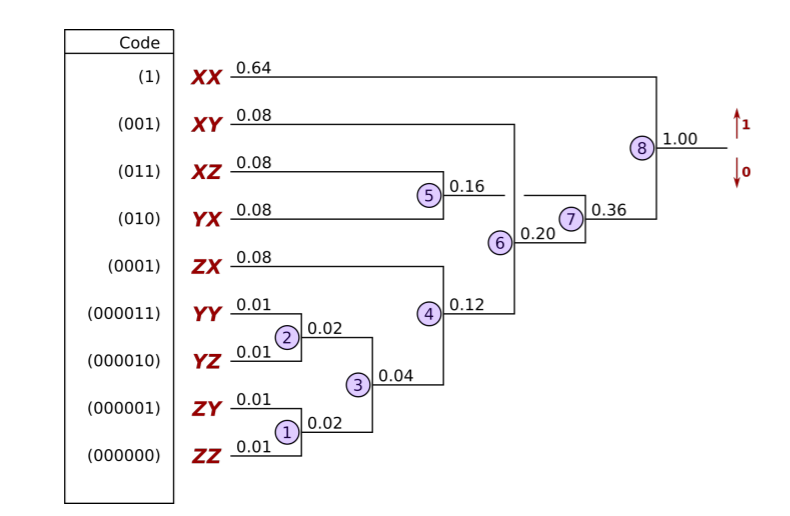
\includegraphics[width=1\linewidth]{images/huffman.png}
\end{align*}

\subsection{LZ77}
Alle Zeichen werden durch Token fixer Länge ersetzt. Token: (Offset, Länge, Zeichen)
\begin{align*}
    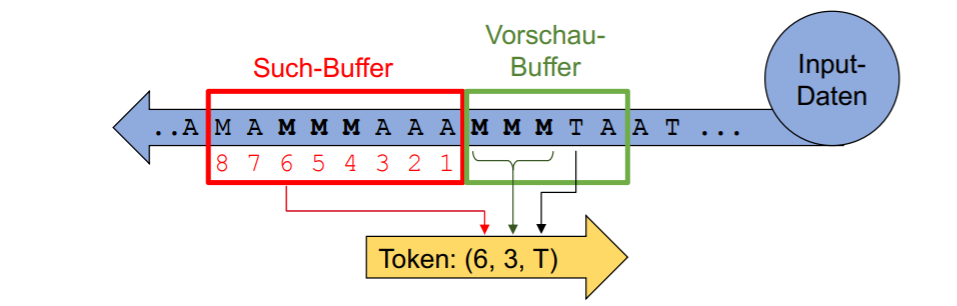
\includegraphics[width=1\linewidth]{images/lz77.png}
\end{align*}

\subsection{LZW}
\begin{enumerate}
    \item Statt einem Sliding Window wird ein Wörterbuch verwendet
    \item Der Index nummeriert die Einträge des Wörterbuchs
    \item Der String bildet den eigentlichen Eintrag
    \item Wörterbuch wird initialisiert mit den möglichen Zeichen resp. Byte-Werten (0..255). à Einzelne Zeichen sind im WB immer vorhanden.
    \item Token enthält nur den Index des schon bestehenden Eintrags im Wörterbuch, nicht aber das zusätzliche Zeichen. Token: (Index)
    \item Das neue Zeichen wird erst mit dem nächsten Token übermittelt (Überlappung)
\end{enumerate}
\textbf{Beispiel: } $\mathtt{A M A M M M A A A M M M T A A T ...}$
\begin{align*}
    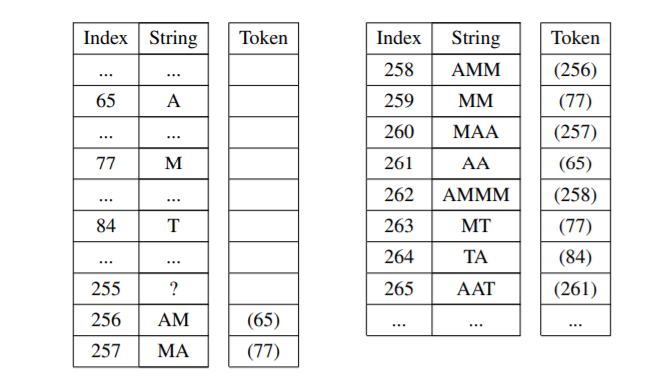
\includegraphics[width=1\linewidth]{images/lzw.png}
\end{align*}

\subsection{Bildkompression - JPEG}

\begin{center}
    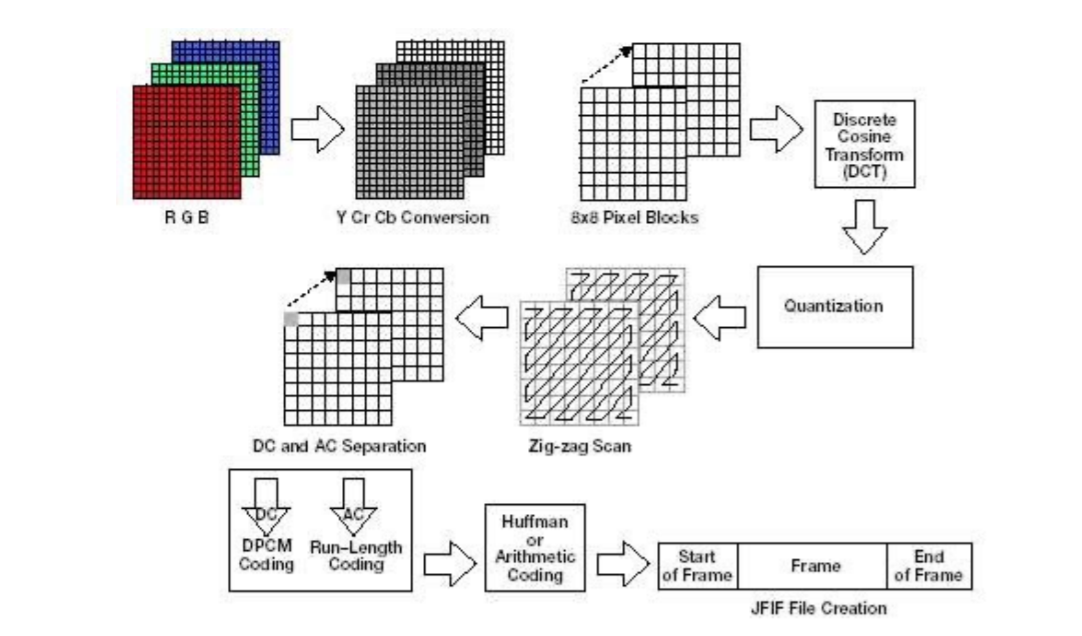
\includegraphics[width=1\linewidth]{images/verfahren.png}
\end{center}

\subsubsection{Kompressionsschritte}%

\begin{enumerate}
    \item Transformation Farbbilder RGB -> Luminanz, Chrominanz
    \item Downsampling der beiden Chrominanz-Komponenten
    \item Pixel-Gruppierung Farbkomponenten in 8x8 Blöcke
    \item Direkte Cosinus Transformation (8x8 DCT)
    \item Individuelle Quantisierung einzelner Frequenzkomponenten
    \item Entropy-Coding der quantisierten Frequenzkomponenten
    \item Erstellen von Header mit JPEG-Parametern
\end{enumerate}

\subsubsection{Luminanz und Chrominanz Farbmodell}

\begin{center}
    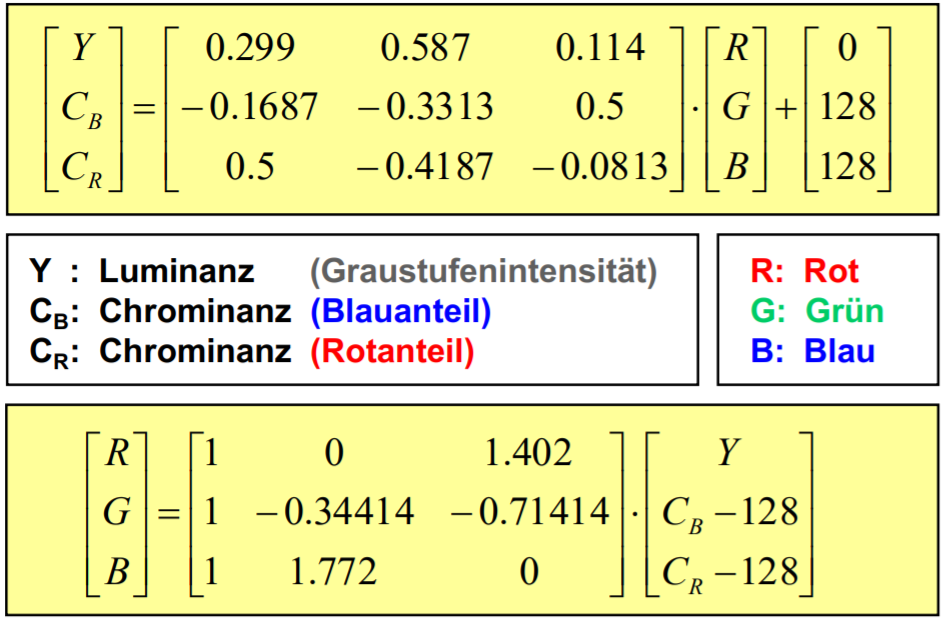
\includegraphics[width=1\linewidth]{images/lumchrom.png}
\end{center}

\subsubsection{Downsampling}

Bei Downsampling werden in beiden Chrominanz-Ebenen in der Horizontalen oder Vertikalen mehrere Pixel zusammengefasst. \\
\textbf{Beispiel: } 4:2:0, 4 bezeichnet hier die Breite des Referenzblocks, 2 bezeichnet wie viele Pixel nach dem Downsampling auf der ersten Zeile und 0 auf der zweiten Zeile vorliegen.
\begin{center}
    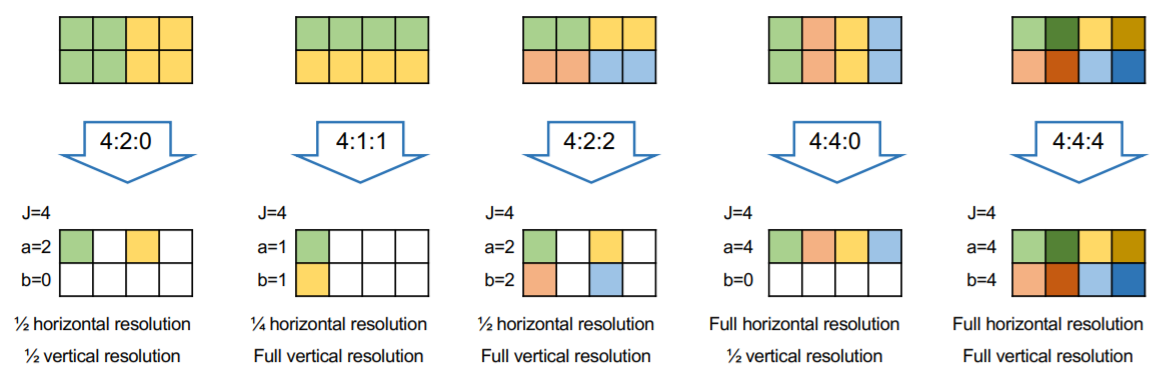
\includegraphics[width=1\linewidth]{images/downsampling.png}
\end{center}

\subsubsection{JPEG Blockverarbeitung}

\begin{center}
    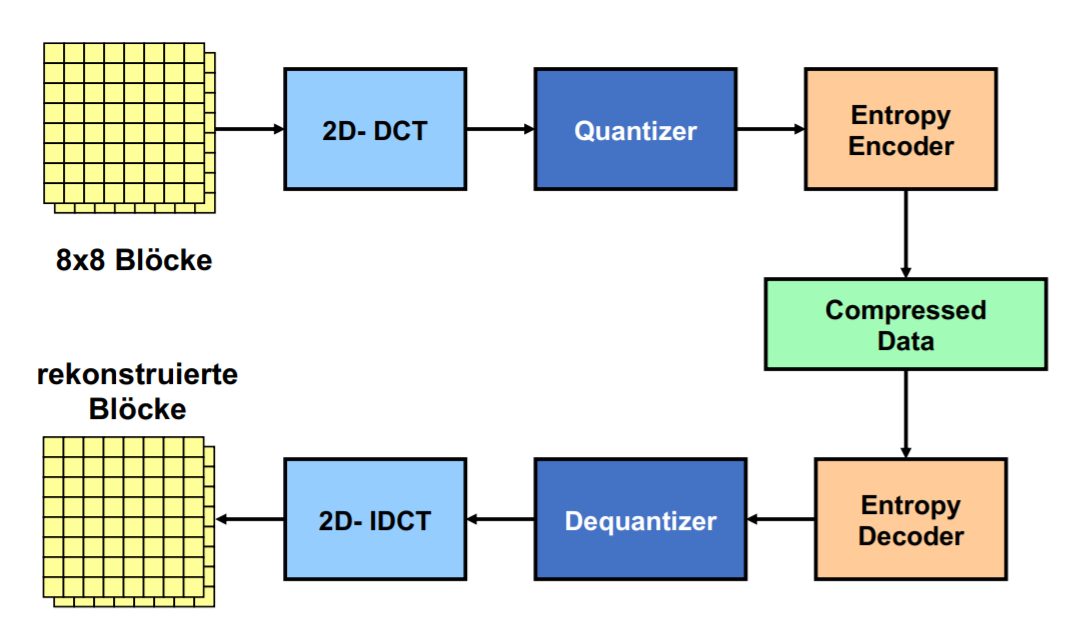
\includegraphics[width=1\linewidth]{images/blockverarbeitung.png}
\end{center}

\subsubsection{DCT Basisfunktion}

\begin{center}
    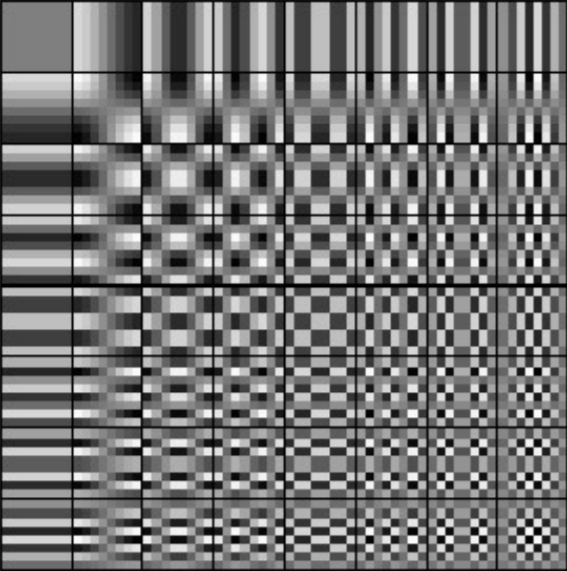
\includegraphics[width=0.6\linewidth]{images/dct.png}
\end{center}

\begin{center}
    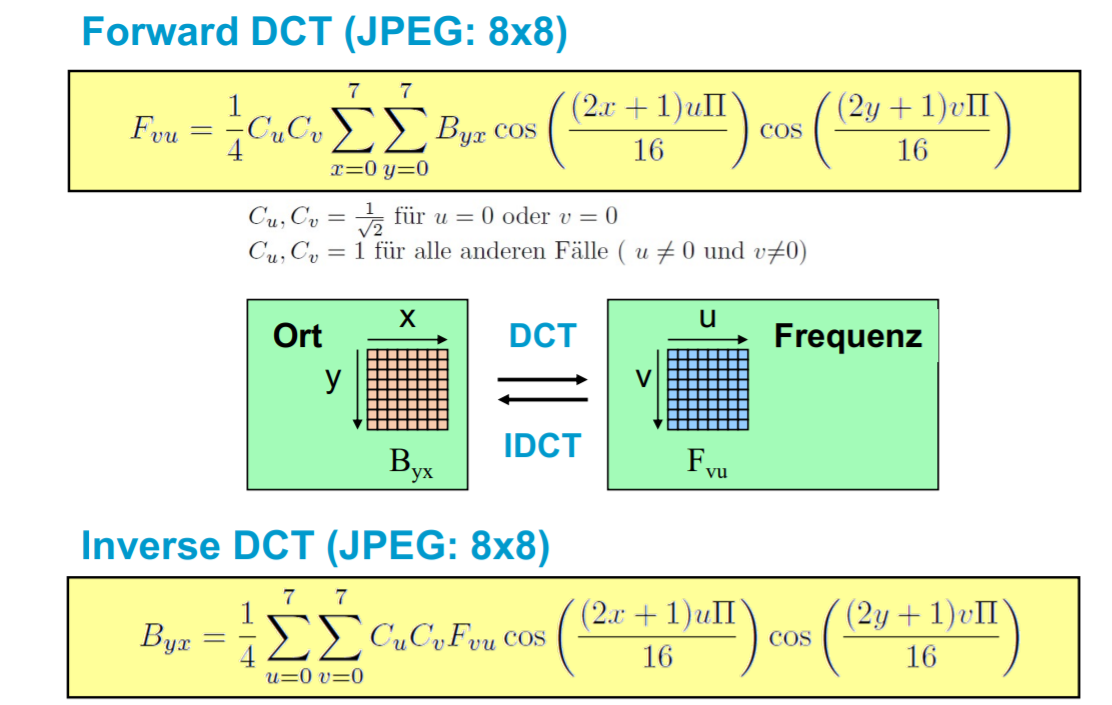
\includegraphics[width=1\linewidth]{images/dctfunction.png}
\end{center}

\begin{center}
    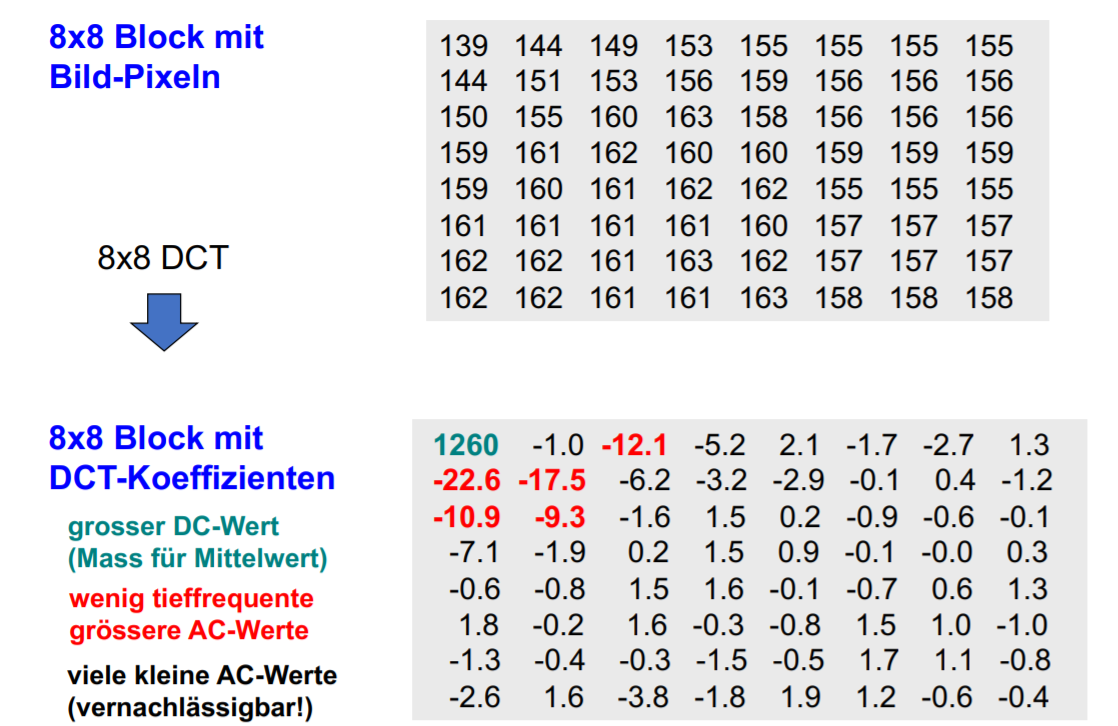
\includegraphics[width=1\linewidth]{images/dctblock.png}
\end{center}

\subsubsection{Quantisierung}%

\begin{center}
    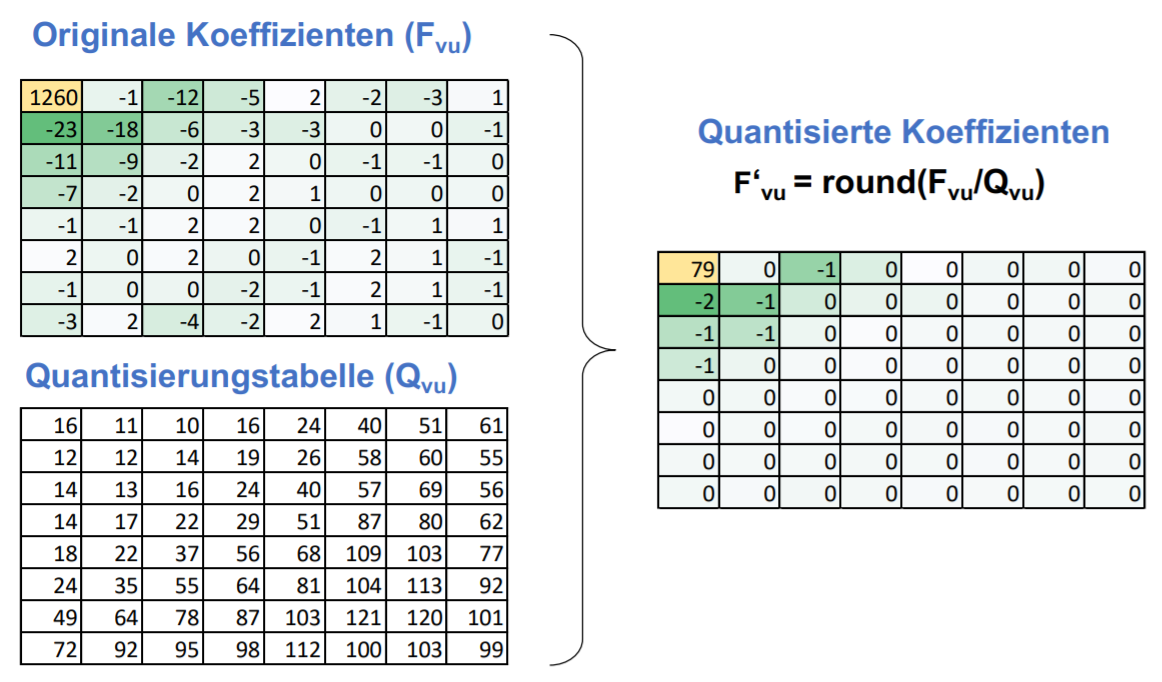
\includegraphics[width=1\linewidth]{images/quantisierung.png}
\end{center}

\subsubsection{Entropy Encoder}

\begin{center}
    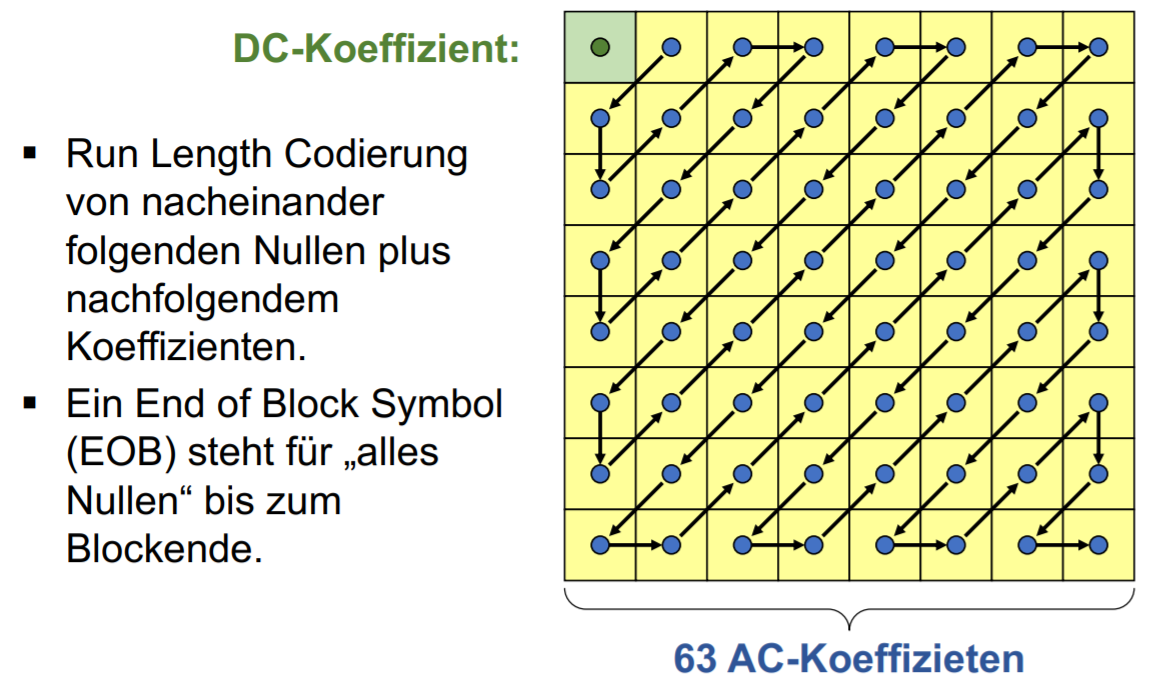
\includegraphics[width=1\linewidth]{images/entropy_encoding.png}
\end{center}

RLE: (DC Wert) (Anzahl Nullen, Koeffizient)...(EOB)

\subsubsection{Dequantisierung}%

\begin{center}
    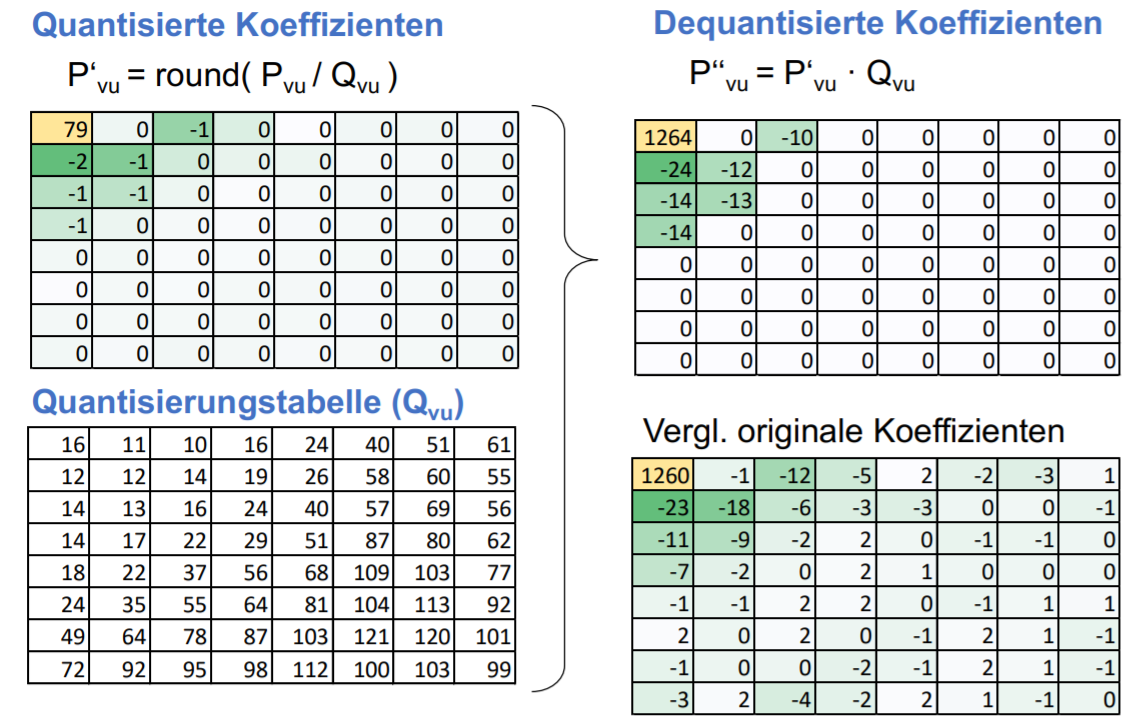
\includegraphics[width=1\linewidth]{images/dequantisierung.png}
\end{center}

\section{Audiocodierung}
\begin{enumerate}
    \item Um ein analoges Audio Signal digitalisieren zu können, muss es abgetastet (sample) und quantisiert werden.
    \item Abtastung bedeutet, dass mit einer bestimmten Abtastfrequenz die Amplitude des Signals gemessen wird.
    \item Quantisierung bedeutet, dass die Amplitude des Signals mit einer bestimmten Anzahl Bits gemessen wird und auf die nächst gelegene Zahl gerundet (quantisiert) wird.
\end{enumerate}

\subsection{Pulse Code Modulation}
\subsubsection{Filterung}
Mit Hilfe eines Filters werden die zu hohen und zu tiefen Frequenzen entfernt. Das Signal wird also auf einen hörbaren Frequenzbereich (20-20kHZ) begrenzt.
\subsubsection{Abtastung}
Die Abtastfrequenz muss mindestens \textbf{doppelt} so gross sein, wir die höchste im analogen Signal vorkommende Frequenz (\textbf{Abtasttheorem von Shannon}).
\subsubsection{Quantisierung}
Die Anzahl Bit, die für die Quantisierung verwendet werden, bestimmt die Anzahl Stufen, welche für die Messung der Amplitude zur Verfügung stehen.
Der Quantisierungsfehler bezeichnet den Fehler, der entsteht wenn die gemessenen Werte gerundet werden.
\subsubsection{Codierung}
Jedem quantisierten Messwert wird ein Wert von einer bestimmten Bitlänge zugeordnet. \textbf{Bitstrom: } Anzahl bits pro Messwert multipliziert mit der Abtastfrequenz.

\subsubsection{Spiegelung}
Bei Eingangssignalen, die grösser sind als die Hälfte der Abtastfrequenz, das "erkannte" Signal an der halben Abtastfrequenz gespiegelt. Bei einer Abtastfrequenz von 8kHz gilt:
\begin{enumerate}
    \item Originalsignal 7kHz -> erkanntes Signal 1kHz
    \item Originalsignal 6kHz -> erkanntes Signal 2kHz
    \item Originalsignal 5kHz -> erkanntes Signal 3kHz
\end{enumerate}

\subsubsection{Quantisierung}%
\textbf{Quantisierungsrauschen: } Differenz Quantisierung <-> Signal. Wird kleiner bei grösser Anzahl verwendeter Bits. Mit jedem Bitanstieg nimmt das Quantisierungsrauschen um 6 dB ab. Jede Bit-Zunahme bedeutet eine Verdoppelung der Anzahl Stufen und damit eine Halbierung des Quantisierungsrauschens.

\begin{center}
    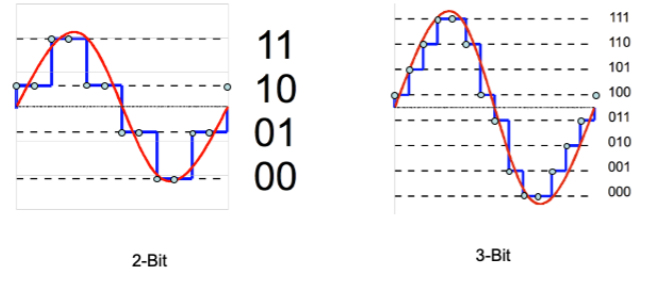
\includegraphics[width=1\linewidth]{images/quantisierungsrauschen.png}
\end{center}

\subsubsection{Lineare Quantisierung}%
Bei einer linearen PCM Codierung wird für jeden Stützwert ein absoluter Wert gemessen und codiert. Dadurch wird bei jedem Stützwert die volle Anzahl Bit für die Quantisierung benötigt.
\begin{center}
    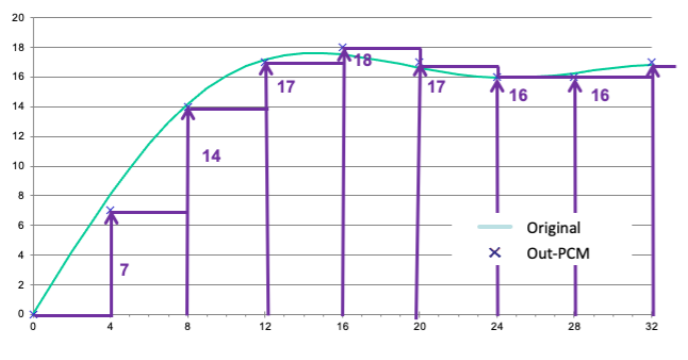
\includegraphics[width=1\linewidth]{images/linearq.png}
\end{center}

\subsubsection{Differential-PCM}%
Bei Differential PCM wird für jeden Stürzwert lediglich die Differenz zum vorherigen Stützwert codiert, was bei Signalfolgen mit geringen Unterschieden - typisch bei digitalen Audiosignalen - zu einer Datenreduktion führt.

\begin{center}
    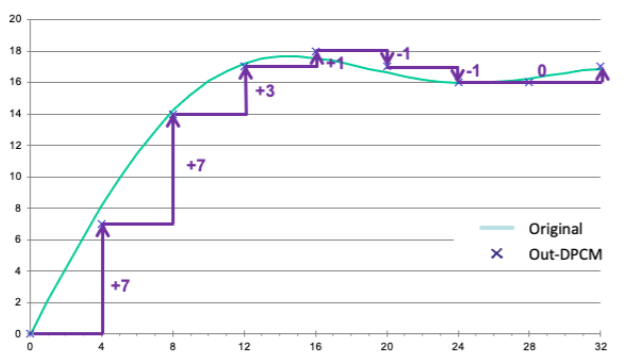
\includegraphics[width=1\linewidth]{images/dpcm.png}
\end{center}

\subsubsection{Adaptive Differential PCM}%
Wird auch Delta Pulse Code Modulation genannt. Wie bei DPCM wird lediglich die Differenz zum vorherigen Stützwert codiert, aber zusätzlich werden nun die Quantisierungsstufen in Abhängigkeit vom Signalverlauf angepasst (adaptiert). Dafür wird ein Korrekturwert K berechnet und nur dieser wird anschliessend übermittelt.
\\
ADPCM ist deshalb ein Codierverfahren mit „Vorhersagefunktion“. Bei der Verarbeitung
des Signals wird versucht, den weiteren Signalverlauf innerhalb des nächsten
Abschnitts vorherzusagen. Für die Quantisierung des Signals im nächsten Zeitschritt
wird so nur die Differenz zwischen vorhergesagtem und realem Signal verwendet. Durch
diese Differenzbildung können so weniger Bits zur Beschreibung des Signals verwendet
werden.
\\
Verfahren: Man misst zuerst die Differenz zum vorherigen Stützwert. Beim nächsten
Stützwert wird die gleiche Differenz (S) noch einmal angewendet und mit dem effektiven
Wert verglichen. Falls der neue Stützwert mit S nicht exakt erreicht wird, wird ein
Korrekturwert K errechnet, um den Wert S so anzupassen, dass die exakte Position
erreicht wird. 
\\
Einerseits können somit gleichbleibende Steigungen mit einer minimalen Anzahl Bit
codiert werden. Andererseits werden zur Beschreibung eines Signals nur die
verhältnismäßig kleinen Korrekturwerte K verwendet, welche mit wenigen Bit
auskommen.
\begin{center}
    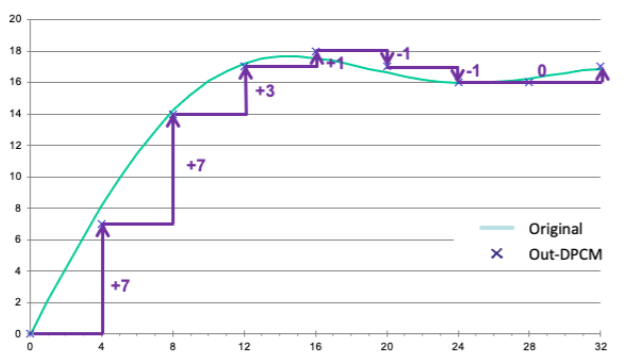
\includegraphics[width=1\linewidth]{images/dpcm.png}
\end{center}

\subsubsection{Linear Prediction Coder LPC}%
\label{ssub:linear_prediction_coder_lpc}

\begin{center}
    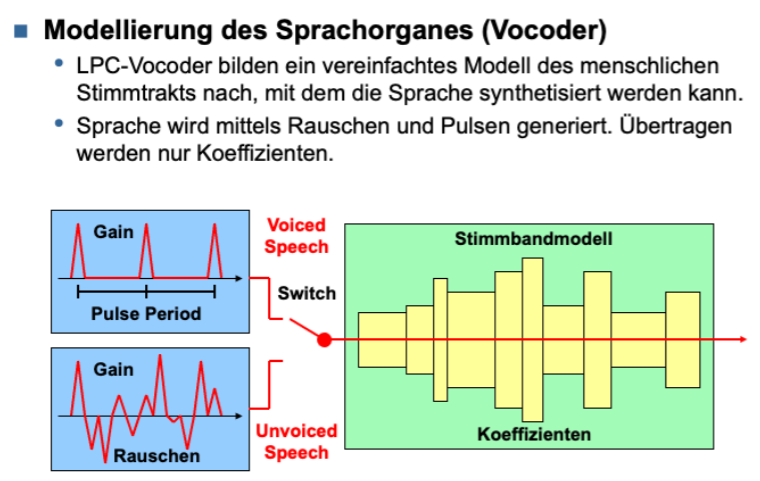
\includegraphics[width=1\linewidth]{images/lpc.png}
\end{center}

\subsection{Wave File Format}%
\label{sub:wave_file_format}

\begin{enumerate}
    \item Containerformat zur digitalen Speicherung von Audiodateien
    \item Basierend auf Microsoft Resource Interchange Format (RIFF)
    \item Wave Dateien enthalten normalerweise keine komprimierten Audiodateien sondern lediglich PCM-Rohdaten
    \item Eine WAVE-Datei enthält vor den Audiodaten einen Header mit Informationen über deren Format
\end{enumerate}

\begin{center}
    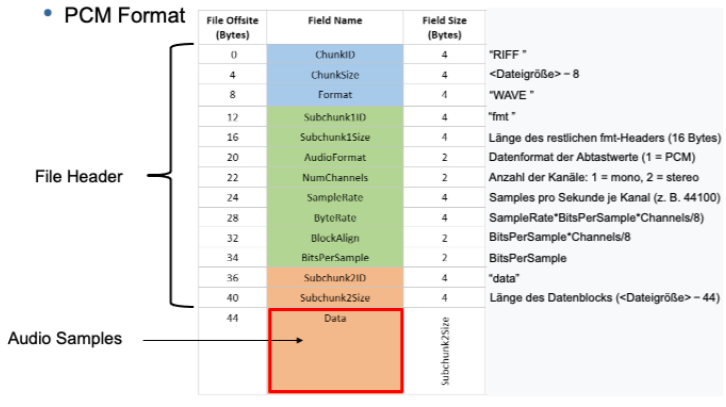
\includegraphics[width=1\linewidth]{images/wave.png}
\end{center}

\begin{center}
    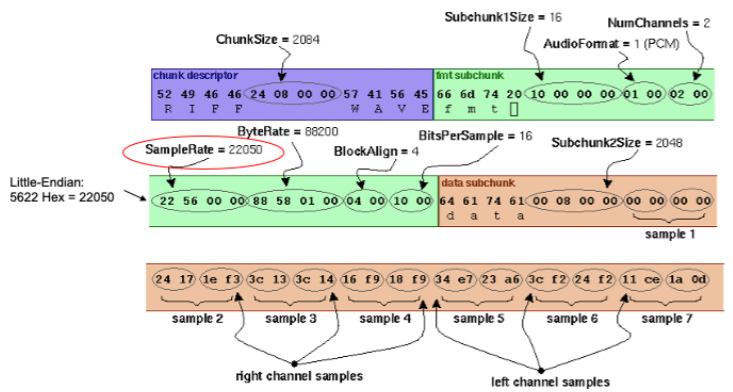
\includegraphics[width=1\linewidth]{images/wavebsp.png}
\end{center}

\subsubsection{Samples}%
\label{ssub:samples}
Die einzelnen Samples $S_i$ für eine gewünschte Frequenz $f$ kann in Abhängigkeit der Abtastrate $R$ und dem Skalierungsfaktor $K$ berechnet werden: $S_i = K \cdot sin(\frac{i \cdot 2 \pi \cdot f}{R})$

Die so erzeugten Samples haben entsprechend ein Intervall von $\frac{2\pi \cdot f}{R}$

\subsubsection{Grösse der Audiodatei}%
\label{ssub:grösse_der_audiodatei}
Header[Byte] + (Abtastfrequenz[Hz] * Dauer[s] + 1) * Auflösung[Byte] * Anzahl Kanäle = [Byte]

\subsection{Schalldruckpegel}%
Schallpegel $L=20 \cdot \log_{10} \frac{p}{p_0}$ Verdoppelung: +6dB.

Der Schalldruckpegel (englisch Sound Pressure Level und oft mit SPL abgekürzt) ist eine
logarithmische Größe zur Beschreibung der Stärke eines Schallereignisses. Der
Schalldruckpegel ist eine berechnete Größe, basierend auf dem Effektivwert des
Schalldrucks.

Der Bezugsschalldruck p0 entspricht der Hörschwelle bei 1kHz und wurde international
normiert auf 0.00002 Pa gesetzt. 

\subsubsection{Menschliche Hörschwelle}%
\label{ssub:menschliche_hörschwelle}

\begin{center}
    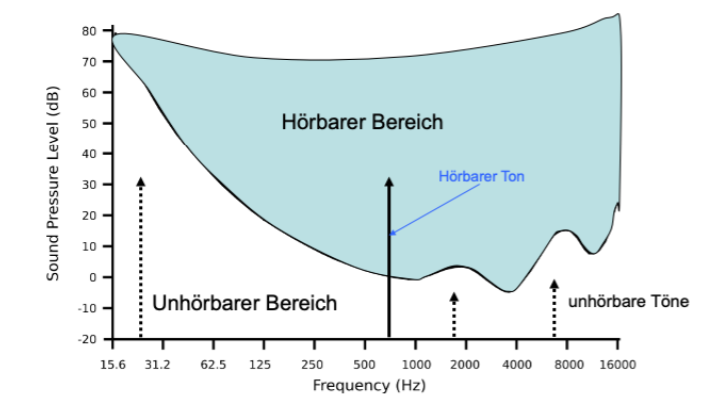
\includegraphics[width=1\linewidth]{images/hoerschwelle.png}
\end{center}

\subsubsection{Maskierung}%
\label{ssub:maskierung}
\begin{enumerate}
    \item Ein lauter Ton kann einen leiseren Ton effektiv maskieren
    \item Je lauter der Ton, desto grösser ist der Frequenzbereich unter- und oberhalb, den er maskieren kann.
    \item Vor-, während und nach einem Ton oder Schallereignis sind leisere Töne nicht hörbar.
\end{enumerate}
\vfill
\subsubsection{Sub-Band Coding}%
\begin{enumerate}
    \item Mehr Bit für die Abtastung -> tieferes Quantisierungs Rauschen
    \item Weniger Bit für die Abtastung -> höheres Quantisierungsrauschen
\end{enumerate}
\begin{center}
    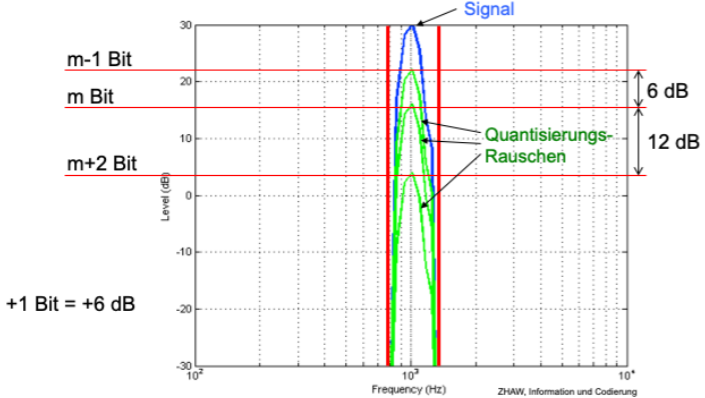
\includegraphics[width=1\linewidth]{images/subband.png}
\end{center}
\begin{center}
    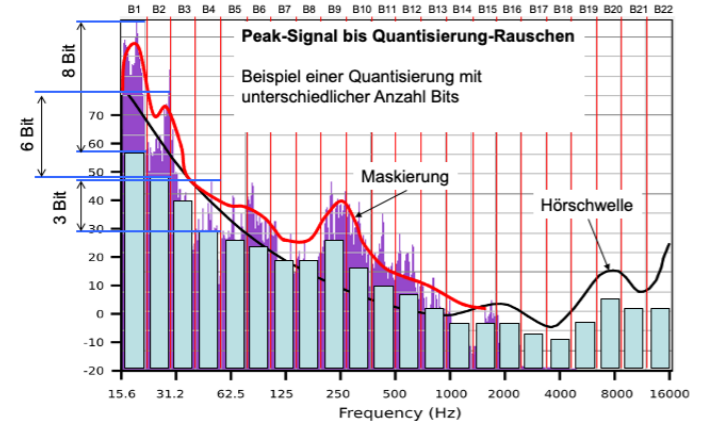
\includegraphics[width=1\linewidth]{images/subband2.png}
\end{center}

\subsection{MPEG Audio}%
\begin{center}
    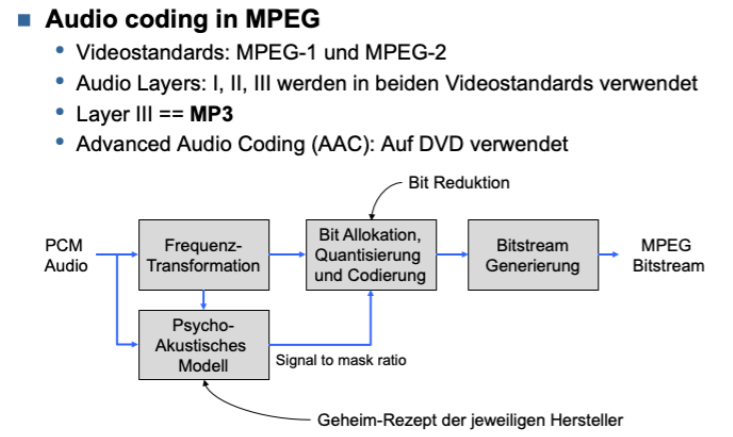
\includegraphics[width=1\linewidth]{images/mpeg.png}
\end{center}
\vfill
